\Chapter{Demo}

%TODO Demozás! Milyen bemenetre milyen kimenetet ad? Következtetések levonása, az összeállított csomag bemutatása
\Aref{tab:obinv_package} táblázatban összefoglalásra kerül a dolgozat eredményiet szemléltető \texttt{obinv} python csomag tartalma.
\begin{table}[h!]
	\centering
	\caption{Az elkészült csomag felépítése}
	\label{tab:obinv_package}
	\medskip
	\scriptsize{
		\begin{tabular}{@{\extracolsep{5pt}} l l p{7.2cm} }
			\hline
			\multicolumn{3}{c}{\textbf{Az \texttt{obinv} csomag tartalma}} \\
			\hline
			\multicolumn{1}{c}{\textbf{Osztály}} & \multicolumn{1}{c}{\textbf{Metódusok}} & \multicolumn{1}{c}{\textbf{Leírás}}\\
			\cline{1-1} \cline{2-2} \cline{3-3}
			\multirow[t]{ 5}{*}{\textit{InputHandler}} & \texttt{remove\_puntuations} & \multirow[t]{ 5}{7.2cm}{A bemeneti szöveg feldolgozásáért felelős osztály. A célja a bemeneti szöveg tisztítása és a tokenek megalkotása.}\\
			& \texttt{make\_lowercase} &\\
			& \texttt{tokenize\_text} &\\
			& \texttt{serialize\_percentage\_tokens} &\\
			\hline
			\multirow[t]{ 2}{*}{\textit{TokenHandler}} & \texttt{compare\_two\_tokens} & \multirow[t]{ 2}{7.2cm}{A tokenek összehasonlító műveleteit megvalósító osztály. A tartalmazás mértékét [0, 1] között adja meg.}\\
			& \texttt{find\_best\_match\_for\_token} &\\
			\hline
			\textit{SynonymsLoader} & \texttt{load\_synonyms} & A \textit{json} formátumban tárolt szinonimák betöltéséért felelős osztály.\\
			\hline
			\multirow[t]{ 4}{*}{\textit{StructuredDataMaker}} & \texttt{find\_classes} & \multirow[t]{ 2}{7.2cm}{A tokenekből való strukturált adatok megalkotásáért felelős osztály. Az osztályokat a szinonima szótár szerint azonosítja. Függősségei a beolvasott szinonima szótár és a \textit{TokenHandler}.}\\
			& \texttt{find\_percentage\_values} &\\
			& \texttt{make\_dict\_from\_classes} &\\
			& \texttt{make\_structured\_data} &\\
			\hline
			\textit{Encoder} & \texttt{make\_one\_hot} & A strukturált adatból one-hot reprezentációt előállító osztály.\\
			\hline
			\textit{ImageSynthetizer} & \texttt{gradient\_descent\_momentum} & A képet előállító osztály, függősége a generátor és a megfelelő osztályozó.\\
			\hline
			\textit{ModelLoader} & \texttt{load\_model} & A betanított modellek betöltéséért felelős osztály.\\
			\hline
			\multirow[t]{ 2}{*}{\textit{ResultPlotter}} & \texttt{show\_result} & \multirow[t]{ 2}{7.2cm}{Az eredmények kirajzolásáért felelős osztály.}\\
			& \texttt{plot\_convergence} &\\
			\hline
			\textit{TextToImage} & \texttt{generate\_image\_from\_text} & A csomag azon osztálya, amely az eddig felsorolt összes funkcionalitáshoz hozzáférést biztosít.\\
			\hline
		\end{tabular}}
\end{table}

\noindent A csomag használatához a \textit{TextToImage} osztály biztosít egy egyszerű elérést, valójában elegendő csupán ezen osztályt beimportálni.

Az alábbi kódrészletekben látható egy példa a csomag használatára:\\
A csomag \textit{TextToImage} osztályát a következőképpen lehet beimportálni és példányosítani. Az osztály használatához szükségeltetik a betanított generátor, a hozzá tartozó osztályozó és a megfelelő szinonima fájl.
\begin{python}
from obinv.TextToImage import TextToImage

generator_path = "./datas/weights/msggan/afhq/msgGenerator.h5"
classifier_path = "./datas/weights/classifier/animalFacesClassifier.h5"
synonyms_path = "./datas/synonyms/afhq_synonyms.json"

animal_text_to_image = TextToImage(generator_path,
                                   classifier_path, synonyms_path)
\end{python}

\noindent A szövegből való kép generálása a következő kódrészlet segítségével történik:
\begin{python}
input_sentence = "Egy macskáról készült fénykép."

step_size = 0.02
momentum = 0.8
steps = 21

result_noises, losses, preds, structured_data =\
    animal_text_to_image.generate_image_from_text(
        input_sentence,
        step_size=step_size, momentum=momentum, steps=steps,
        verbose=True, show_convergence=True
    )
\end{python}

Mivel a kép generálásában a véletlenszerű tényező igen nagy, így egy bemeneti mondatra a futtatások során egymástól eltérő képek kerülnek kigenerálásra. A fenti kódrészleteket futtatva a \ref{fig:demo} ábrához hasonló figyelhető meg.

\begin{figure}[h]
	\centering
	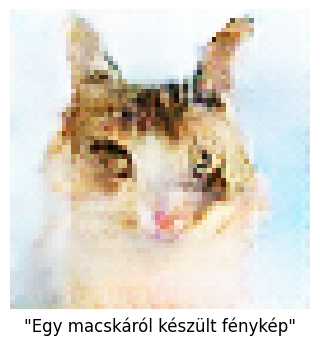
\includegraphics[width=6cm]{images/demo01.png}
	\caption{Példa egy futtatás eredményére}
	\label{fig:demo}
\end{figure}

Amennyiben a \texttt{generate\_image\_from\_text} függvény \texttt{show\_convergence=True} paraméter értékkel kerül futtatásra, úgy a \ref{fig:demo_convergence} ábrához hasonló kimenetet is kaphatunk. Az ábrán megfigyelhetjük, hogy a programnak milyen úton sikerült kigenerálnia a kimeneti képet. A bal felső sarokban a hibafüggvény változását figyelhetjük meg a lépések során. Jobb felső sarokban az egyes lépésekhez tartozó kigenerált képen azonosított címkék valószínűségi értékeinek változását követhetjük nyomon. Az ábra alján pedig az egyes lépésekhez tartozó generált képeket lehet megfigyelni.

\begin{figure}[h]
	\centering
	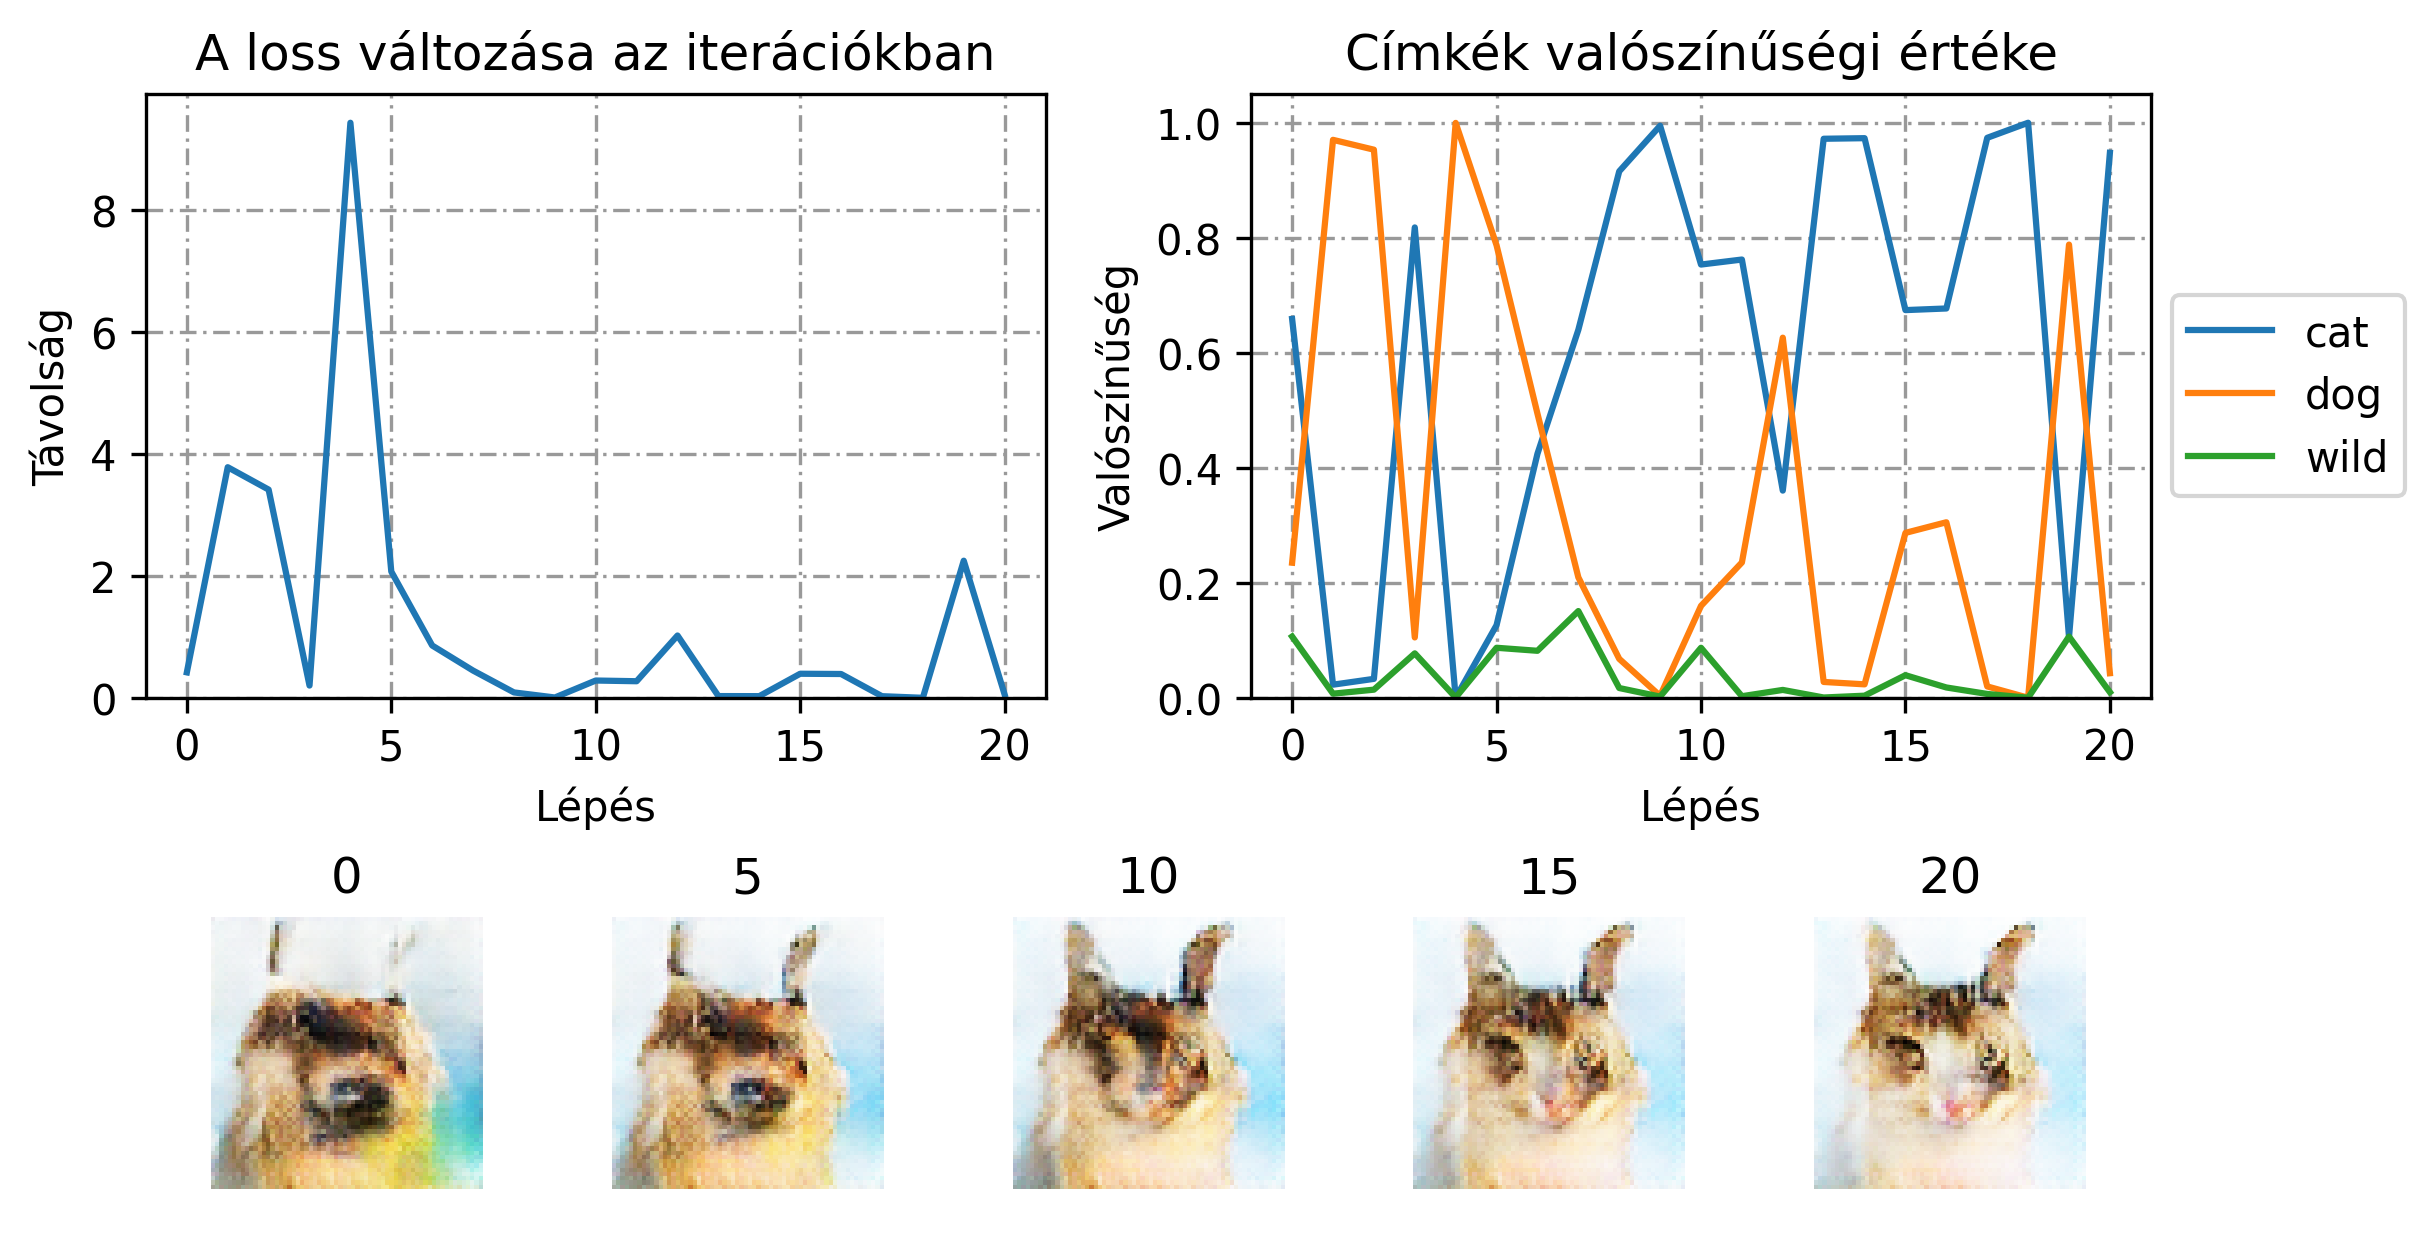
\includegraphics[width=15cm]{images/demo01_conv.png}
	\caption{A példa kép közelítése a lépésekben}
	\label{fig:demo_convergence}
\end{figure}

A kimeneti kép jósága sok paramétertől függhet, illetve a generálás kiinduló pontja is nagymértékben befolyásolja az eredményt. Mivel a pont egy véletlenszám generátorral kerül meghatározásra, így egy megadott seed értékkel beállítható a kiinduló pont. A seed értéket a \texttt{generate\_image} függvény paramétereként lehet megadni.

A \textit{TextToImage} osztály \texttt{generate\_image\_from\_text} függvényének paraméterei a következők:

\begin{itemize}
	\item \textbf{input\_text}: A bemeneti szöveg, amely egy leírómondat a kép tartalmára illetőleg.
	\item \textbf{step\_size}: A gradiens keresésben alkalmazott lépésköz értéke. Default érték = \texttt{0.005}.
	\item \textbf{momentum}: A gradiens keresés momentum értéke. Default érték = \texttt{0.9}.
	\item \textbf{steps}: A gradiens keresés ismétlésszáma. Default érték = \texttt{21}.
	\item \textbf{seed}: A kiinduló random pont seed értéke. Default = \texttt{None}
	\item \textbf{image\_step}: A konvergencia ábrára rajzolt képek közti lépésköz. Default érték = \texttt{5}.
	\item \textbf{dpi}: A kirajzolandó kimeneti képek dpi értéke. Default érték = \texttt{100}.
	\item \textbf{verbose}: \texttt{True} érték esetén a keresés minden lépésének kimenete megjelenik. Default érték = \texttt{False}.
	\item \textbf{show\_convergence}: \texttt{True} érték esetén kirajzolásra kerül a konvergencia ábra. Default érték = \texttt{False}.
\end{itemize}

A függvénynek csupán egyetlen kötelező paramétere van, a bemeneti mondat. A további paraméterek megadása opcionális.

A kódrészletben is látható, hogy a függvénynek négy visszatérési van: \texttt{result\_noises}, \texttt{losses}, \texttt{preds}, \texttt{structured\_data}. Valójában az első három érték a konvergencia ábrán megjelenítésre kerül, sorrendben: a keresés soránt talált zajok (amelyekből a képek előállíthatóak), a hiba értékek és az osztályozó kimenetei a keresés alatt. Ezen értékeket csupán az esetleges további vizsgálatok érdekében kerülnek visszatérésre. A \texttt{structured\_data} érték pedig a szöveg feldolgozás során kapott strukturált adat.
A fenti példa futtatásra előállt strukturált adat a következő:
\begin{verbatim}
{'cat': 1.0, 'dog': 0.0, 'wild': 0.0}
\end{verbatim}

\Section{Példafuttatások}

\begin{verbatim}
input_sentence = "Egy macskutyáról képszült felvétel."

step_size = 0.02
momentum = 0.9
steps = 21
{'cat': 0.5, 'dog': 0.5, 'wild': 0.0}
\end{verbatim}

\begin{figure}[h]
	\centering
	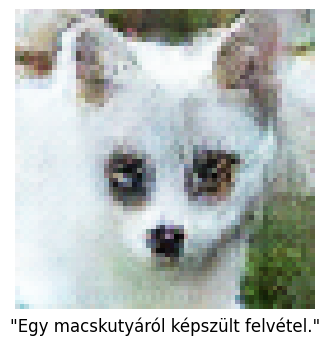
\includegraphics[width=6cm]{images/demo02.png}
	\caption{Második példa}
	\label{fig:demo2}
\end{figure}

\begin{figure}[h]
	\centering
	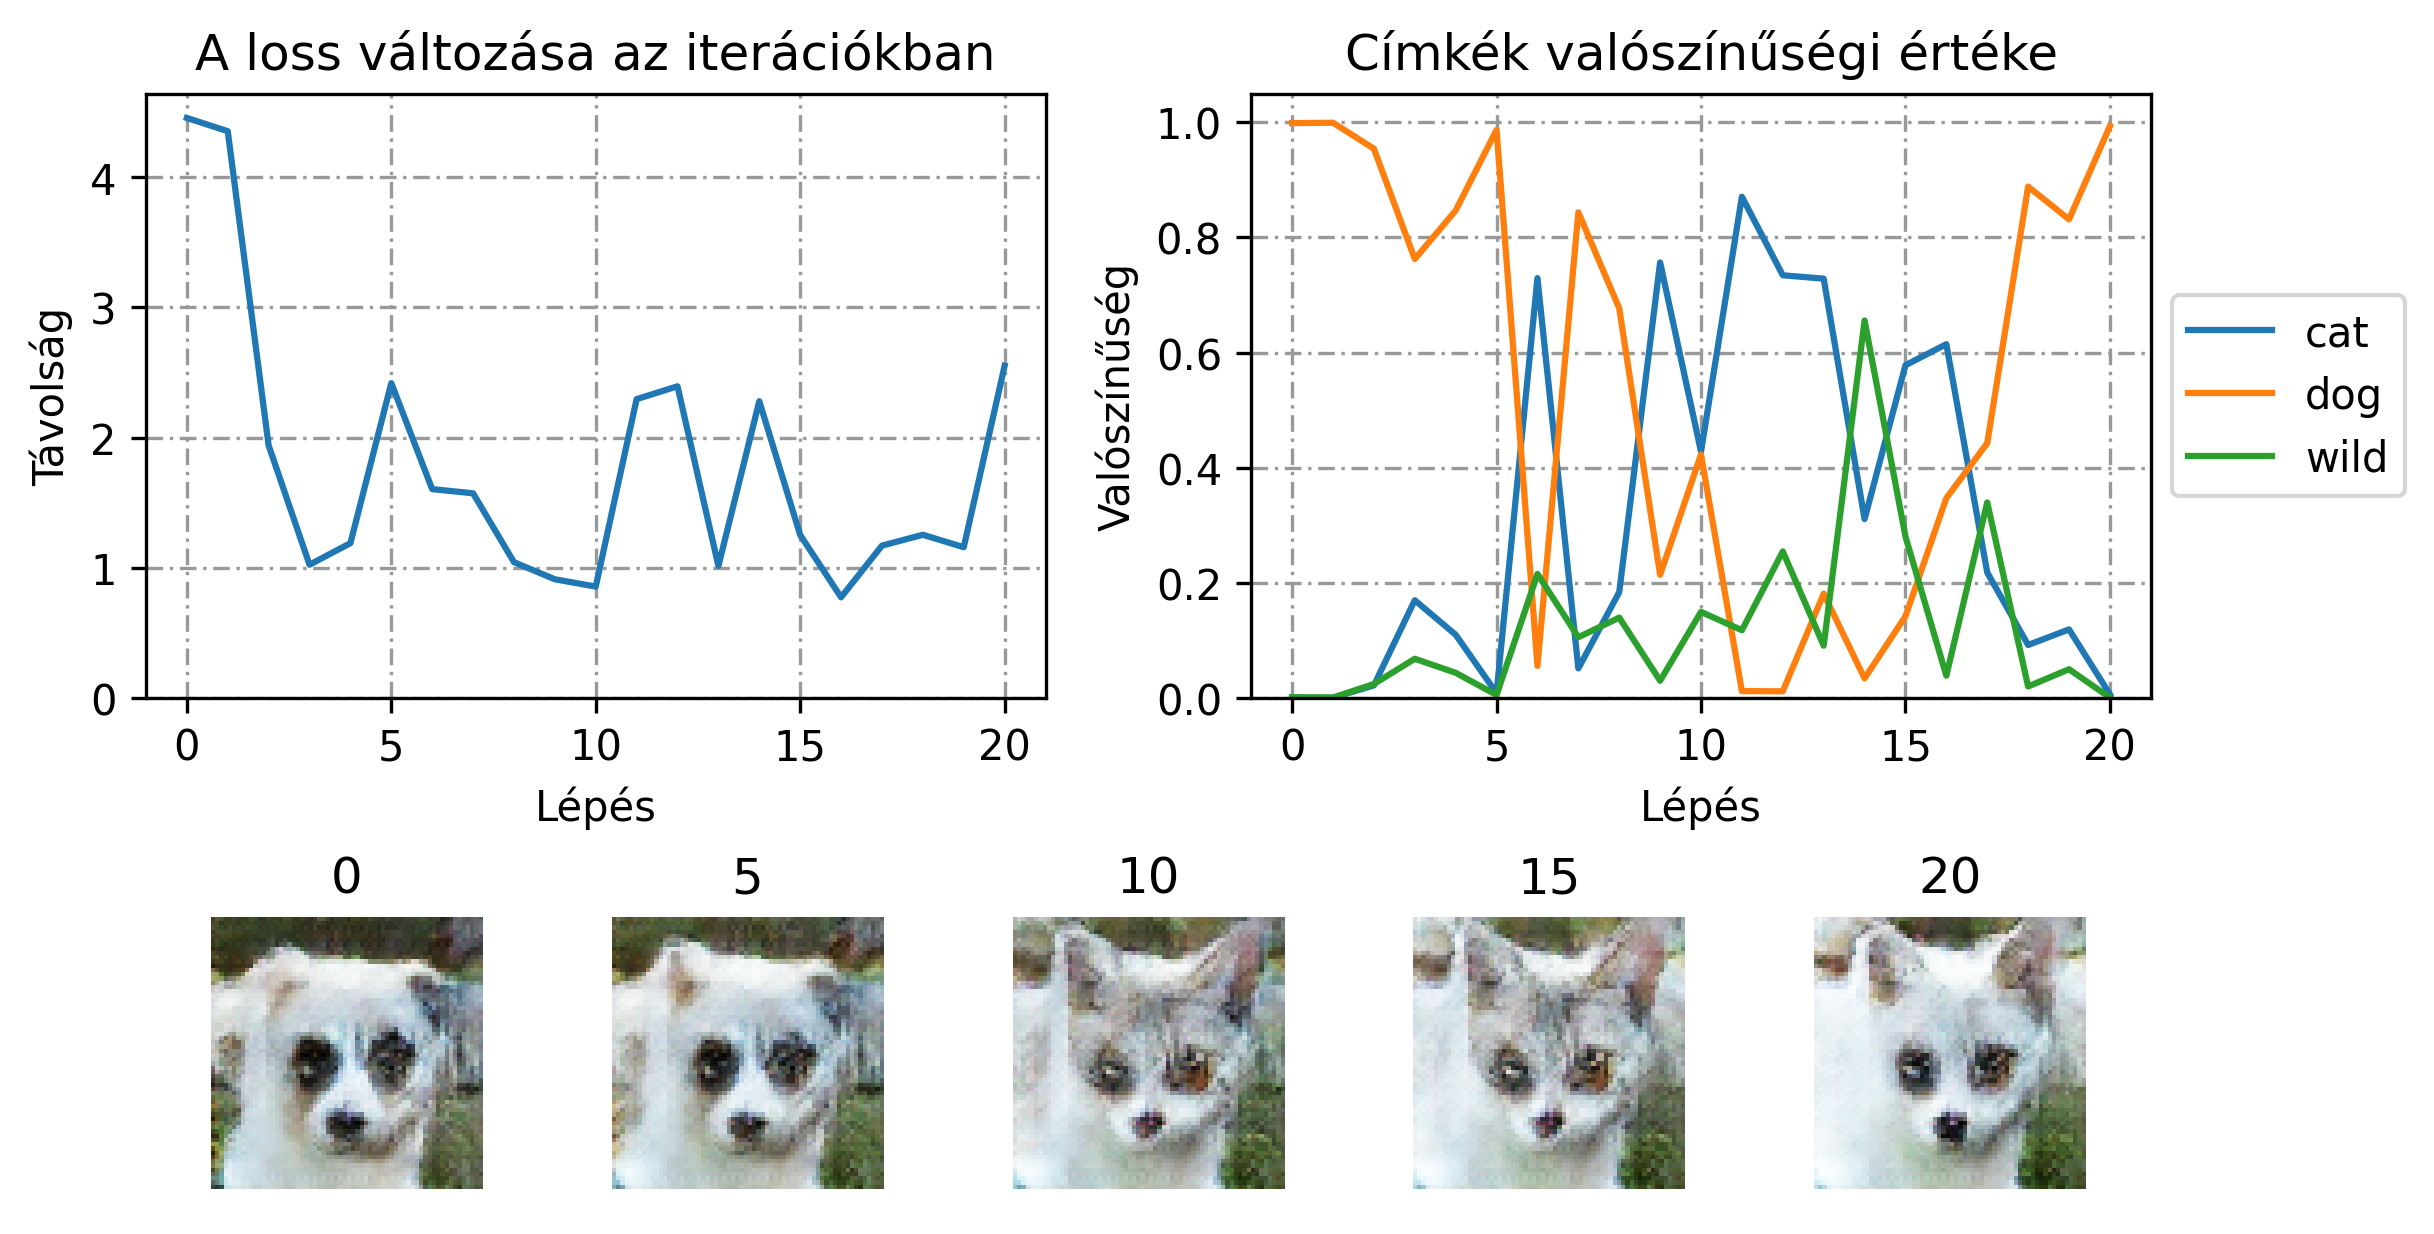
\includegraphics[width=15cm]{images/demo02_conv.png}
	\caption{A második példa kép közelítése a lépésekben}
	\label{fig:demo2_convergence}
\end{figure}

A \ref{fig:demo2} ábrán egy olyan példa figyelhető meg, amelyben kevert osztály kikeresése volt a cél. Az eredményen látható, hogy a kiinduló kép kutyaként lett osztályozva, majd a keresés során a macska osztályra jellemző tulajdonságok fokozatosan megjelennek: a kutya füle és bundájának mintázata a macska osztályból ismert tulajdonságokat veszi fel. Mindezek mellett az orr és a szemek közti foltok megmaradnak.

\begin{verbatim}
input_sentence ="Egy olyan ló, amely 20%-ban agancsos"
step_size = 0.02
momentum = 0.8
steps = 21
{'airplane': 0.0, 'automobile': 0.0, 'bird': 0.0, 'cat': 0.0, 'deer': 0.2,
 'dog': 0.0, 'frog': 0.0, 'horse': 0.8, 'ship': 0.0, 'truck': 0.0}
\end{verbatim}

\begin{figure}[h]
	\centering
	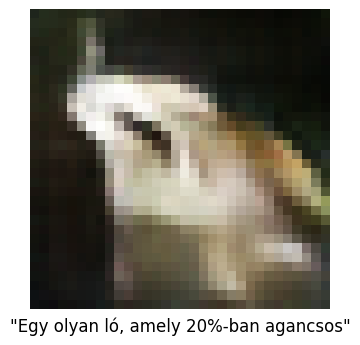
\includegraphics[width=6cm]{images/demo03.png}
	\caption{Harmadik példa}
	\label{fig:demo3}
\end{figure}

\begin{figure}[h]
	\centering
	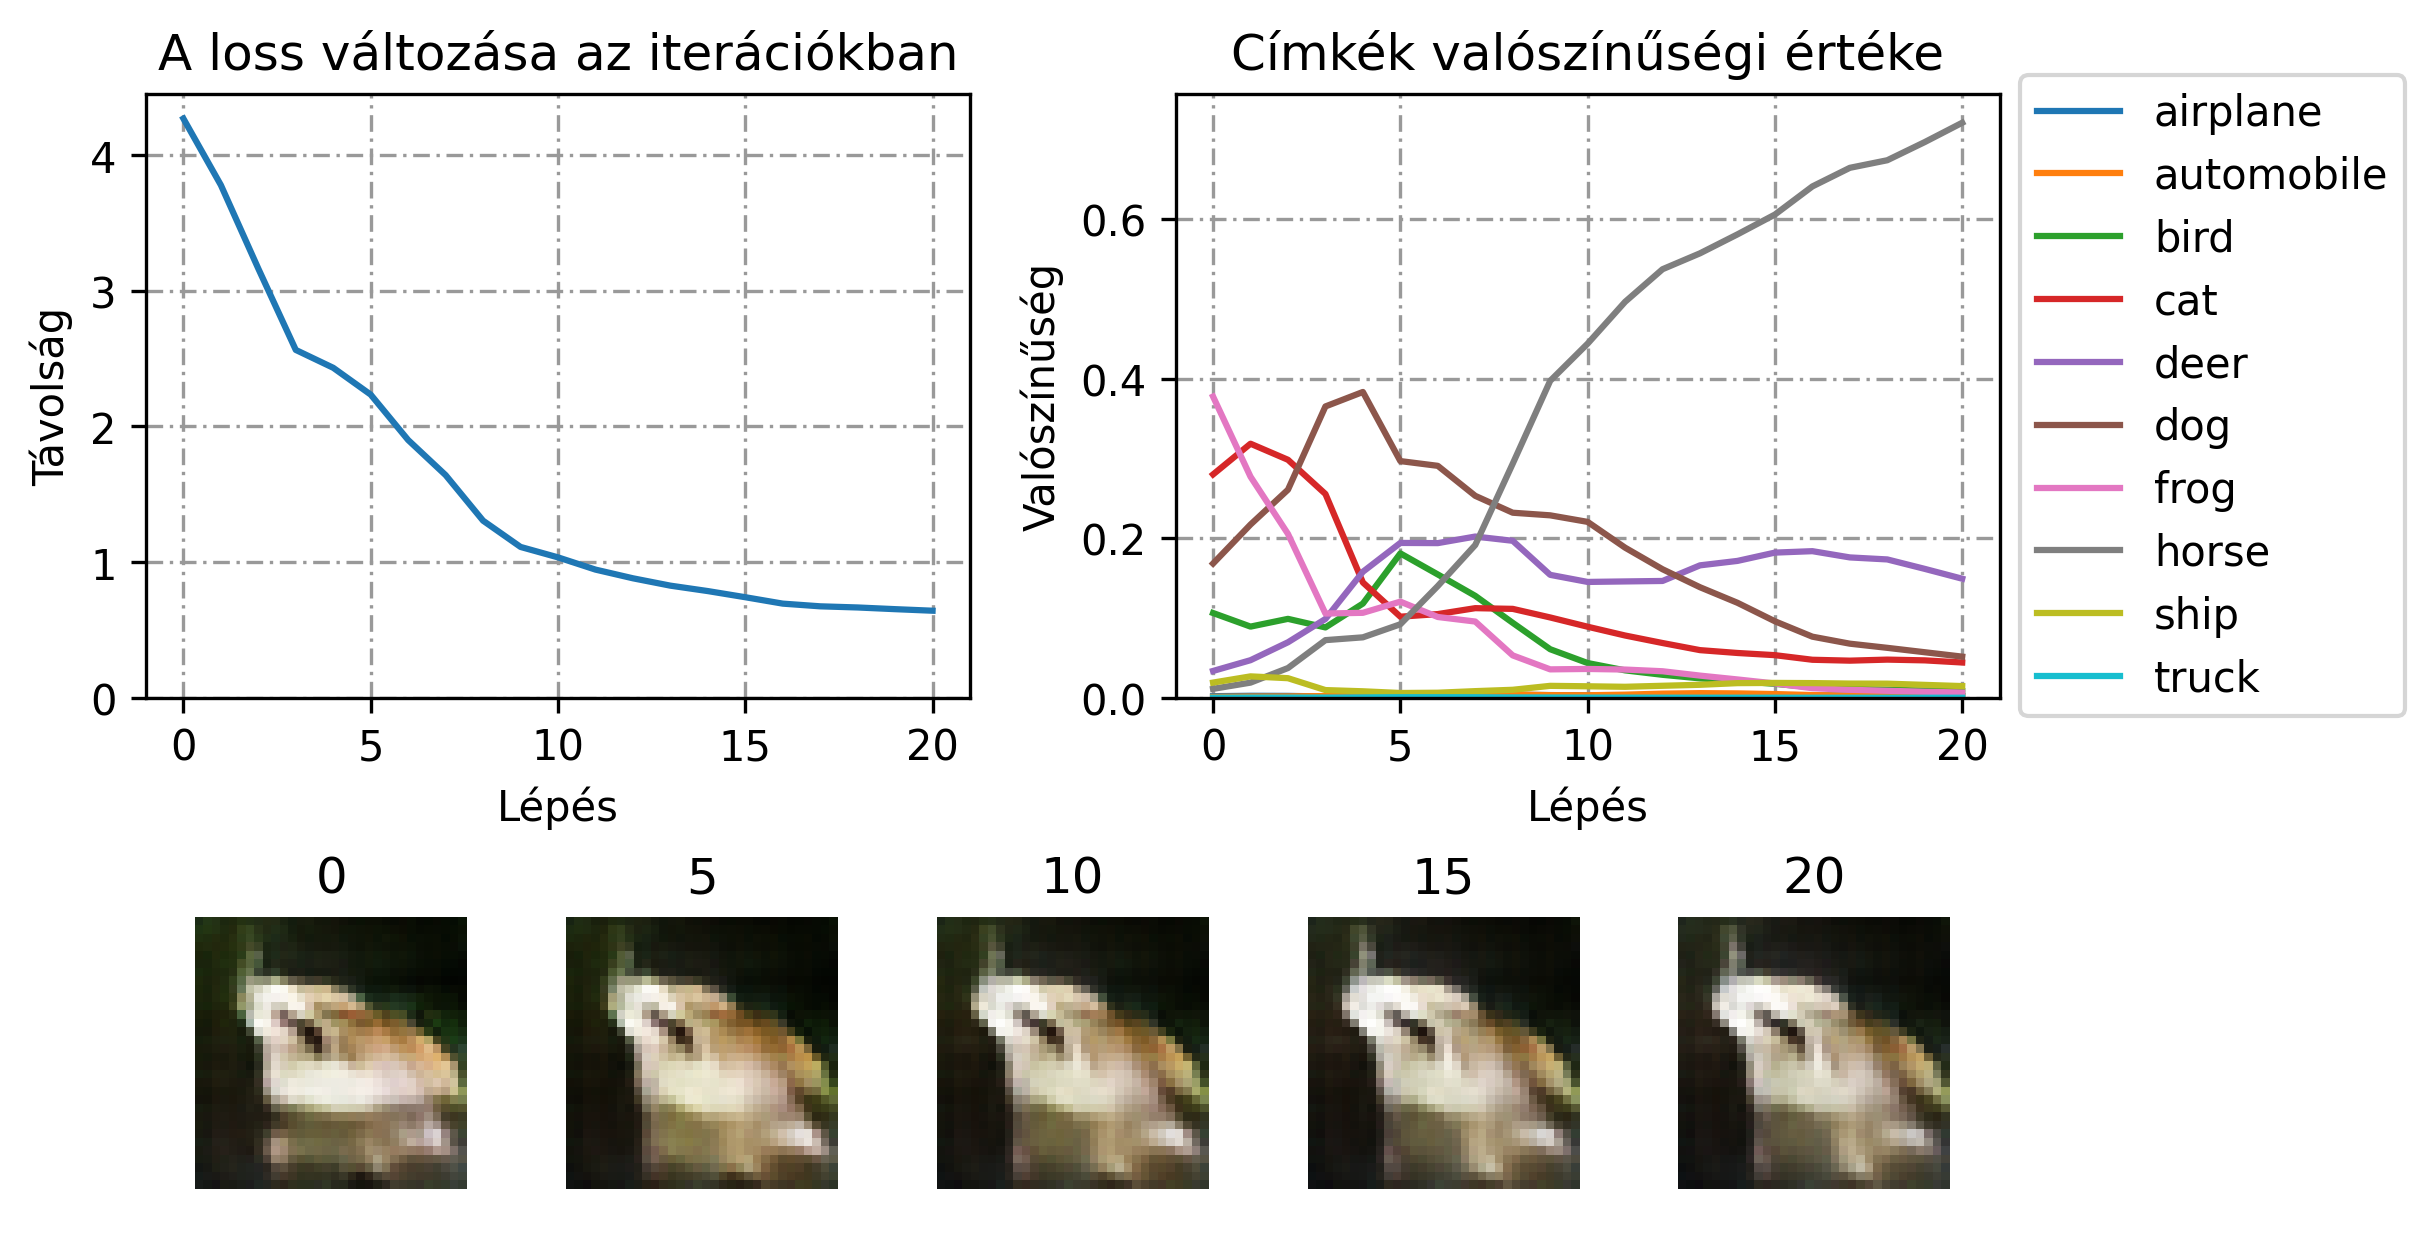
\includegraphics[width=15cm]{images/demo03_conv.png}
	\caption{A harmadik példa kép közelítése a lépésekben}
	\label{fig:demo3_convergence}
\end{figure}

A \ref{fig:demo3} ábrán látható kimenet a \ref{fig:demo3_convergence} konvergencia görbék alapján megfelelően kigenerálódott. A köztes képeket vizsgálva valójában nem sok változás történt a kiinduló és a talált kép között. Viszont a leíró mondatnak az osztályozó szerint ezen kimeneti kép felelt meg a legjobban. A Cifar10 adathalmaz 10 darab osztálya már kisebb kihívást jelenthet ezen módszernek. A kiinduló képtől nagy mértékben függ a kimenet.

\begin{verbatim}
input_sentence = "Egy hajó a tengeren"
step_size = 0.03
momentum = 0.8
steps = 21
{'airplane': 0.0, 'automobile': 0.0, 'bird': 0.0, 'cat': 0.0, 'deer': 0.0,
 'dog': 0.0, 'frog': 0.0, 'horse': 0.0, 'ship': 1.0, 'truck': 0.0}
\end{verbatim}

\begin{figure}[h]
	\centering
	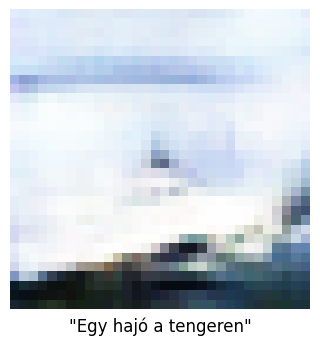
\includegraphics[width=6cm]{images/demo04.png}
	\caption{Negyedik példa}
	\label{fig:demo4}
\end{figure}

\begin{figure}[h]
	\centering
	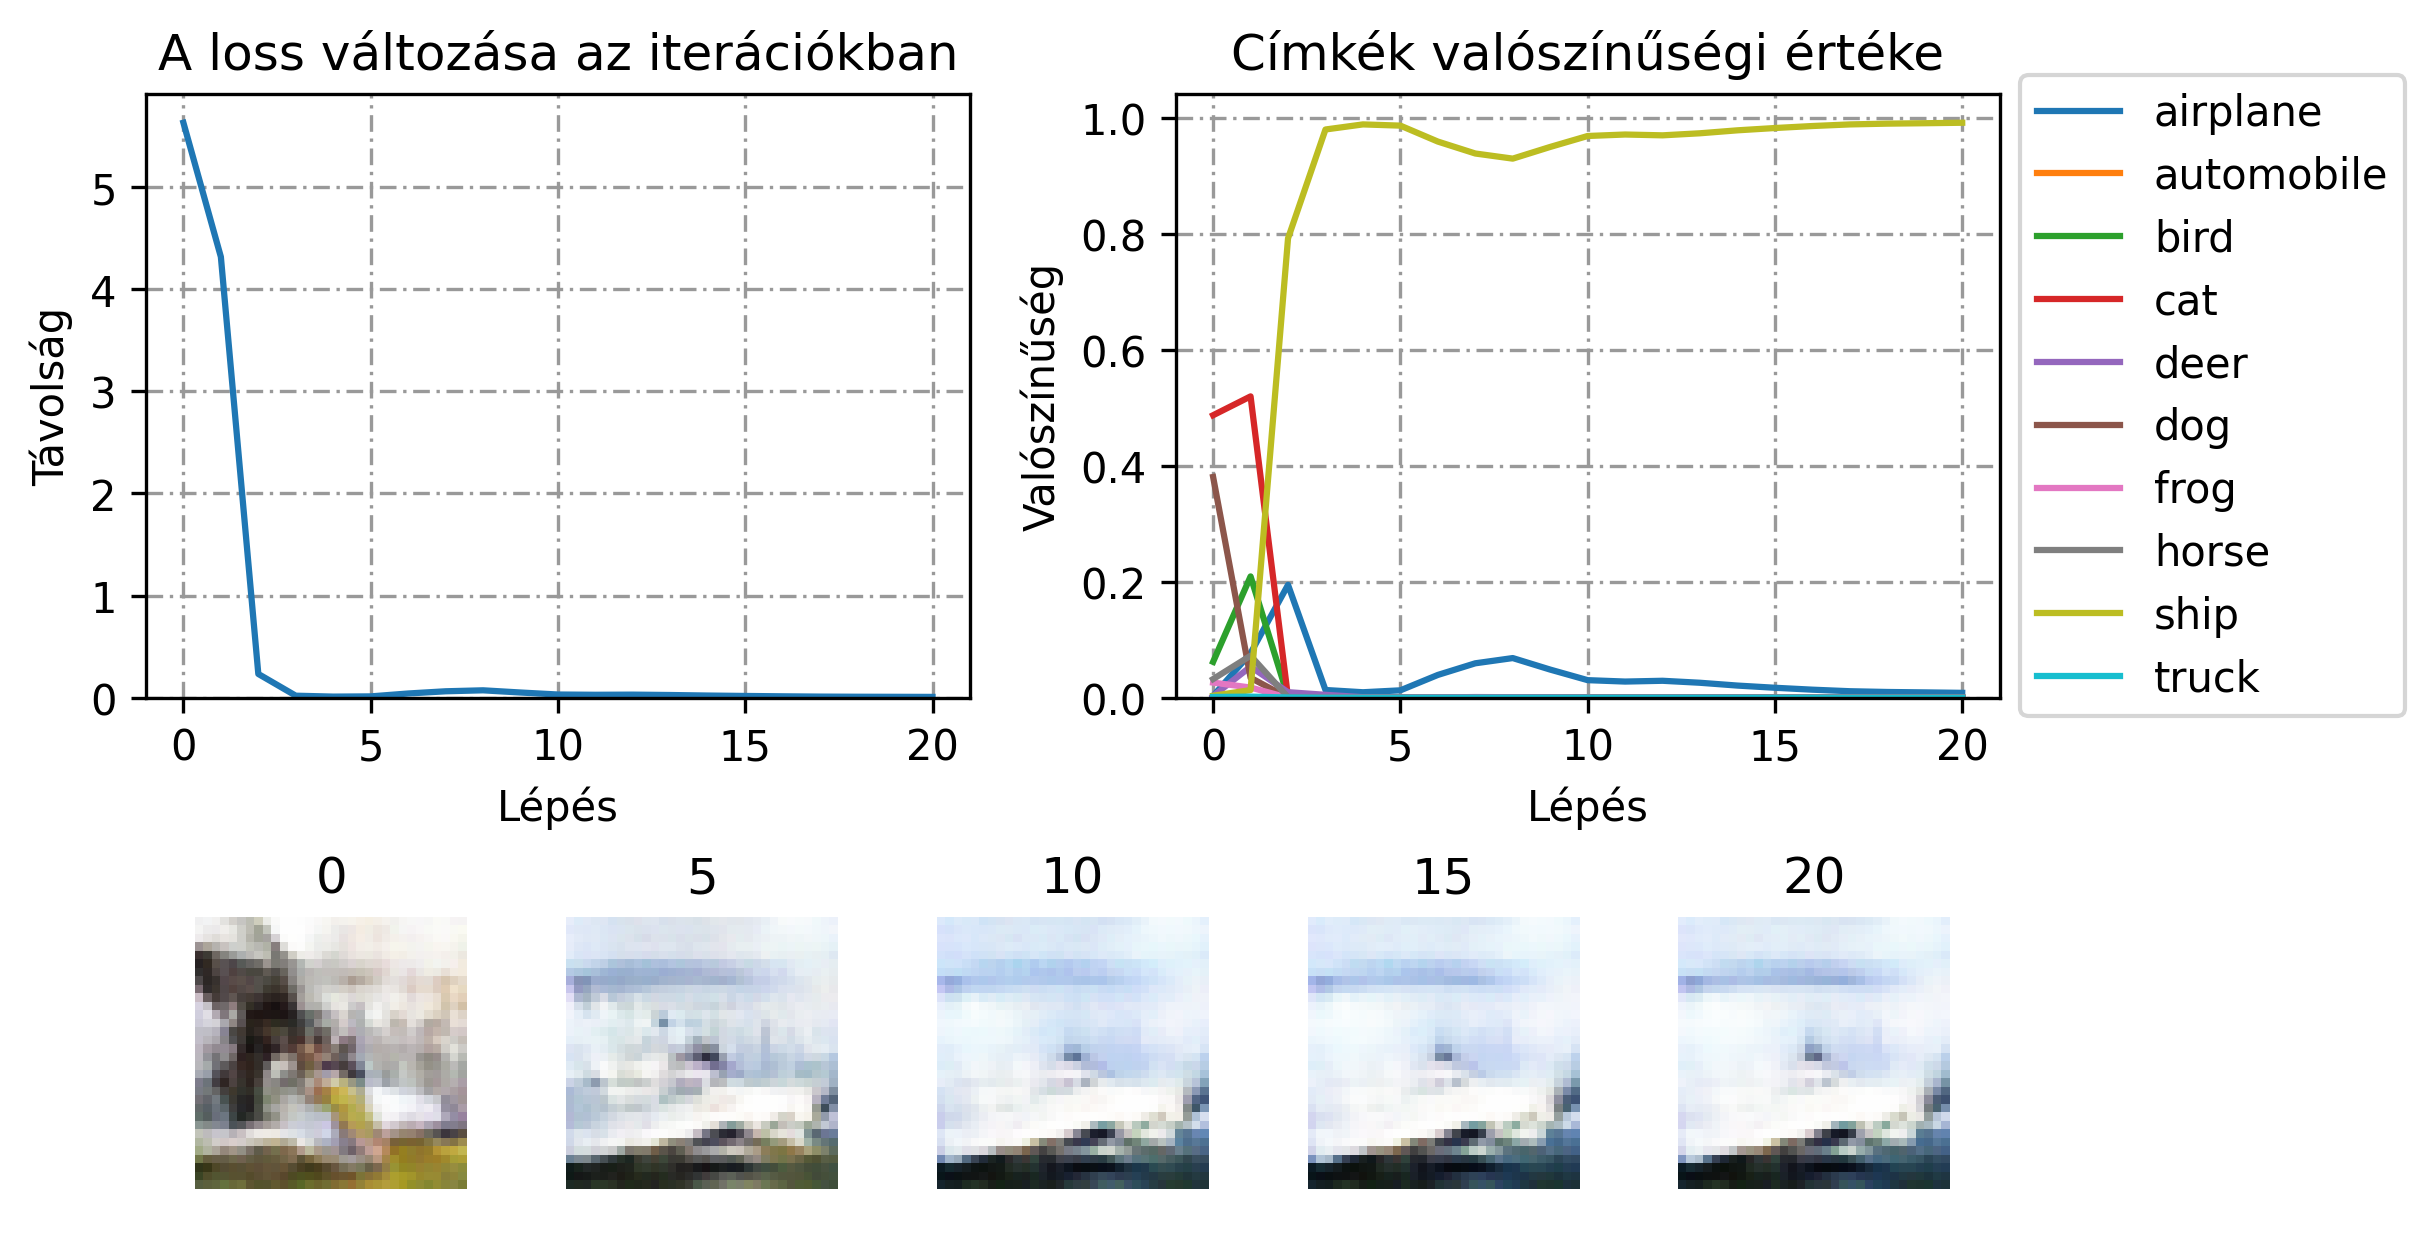
\includegraphics[width=15cm]{images/demo04_conv.png}
	\caption{A negyedik példa kép közelítése a lépésekben}
	\label{fig:demo4_convergence}
\end{figure}

A \ref{fig:demo4_convergence} ábrán megfigyelhető, hogy a példában igazán hamar megtalálta a módszer a megfelelő képet, amely után már csupán igen kis mértékű változásokat eszközölt.

A kapott végeredmények igen sok paramétertől függnek. Nem csupán a program futtatása során megadott értékek, mint a lépésköz és momentum van hatással az eredményre. Az osztályozó és a generátor tanítása is igen sok paramétertől függvényében történik és így ezen komponensek jósága kritikus a keresés szempontjából.